\thispagestyle{empty}
\global\watermarkfalse
\begin{tikzpicture}[remember picture,overlay]
  \coordinate (C) at (current page.center);
  % ivory board with soft burgundy surround
  \fill[navy] (current page.south west) rectangle (current page.north east);
  \fill[ivory] ($(current page.south west)+(1.0cm,1.0cm)$) rectangle ($(current page.north east)+(-1.0cm,-1.0cm)$);
  \shade[inner color=ivory,outer color=softgilt!70,opacity=0.9] ($(current page.south west)+(1.0cm,1.0cm)$) rectangle ($(current page.north east)+(-1.0cm,-1.0cm)$);
  % ornate triple gold frame
  \draw[gilt,line width=2.4pt] ($(current page.south west)+(1.35cm,1.35cm)$) rectangle ($(current page.north east)+(-1.35cm,-1.35cm)$);
  \draw[gilt,line width=0.6pt] ($(current page.south west)+(1.6cm,1.6cm)$) rectangle ($(current page.north east)+(-1.6cm,-1.6cm)$);
  \draw[navy,line width=0.4pt] ($(current page.south west)+(1.75cm,1.75cm)$) rectangle ($(current page.north east)+(-1.75cm,-1.75cm)$);
  \foreach \p/\s in {north west/none,north east/v,south west/h,south east/c}{
    \node[inner sep=0pt,anchor=\p] at ($(current page.\p)+(\ifnum\pdfstrcmp{\p}{north west}=0 1.8\else\ifnum\pdfstrcmp{\p}{south west}=0 1.8\else -1.8\fi\fi cm,\ifnum\pdfstrcmp{\p}{north west}=0 -1.8\else\ifnum\pdfstrcmp{\p}{north east}=0 -1.8\else 1.8\fi\fi cm)$)
      {\pgfornament[width=2.6cm,color=gilt,symmetry=\s]{41}};}
  % top flourish and crest
  \node[inner sep=0pt] at ($(current page.north)+(0,-2.35cm)$) {\pgfornament[width=7cm,color=gilt]{87}};
  \node[inner sep=0pt] (crest) at ($(current page.north)+(0,-6.2cm)$) {
\includegraphics[width=6.2cm]{img/logo}};
  \draw[gilt,line width=1.2pt] (crest.center) circle (3.25cm);
  \draw[navy,line width=0.4pt] (crest.center) circle (3.4cm);
  % title block
  \node[align=center,text width=15cm] at ($(current page.north)+(0,-12.6cm)$) {%
    {\color{gilt}\scshape\large Science Monk \textperiodcentered{} Presents}\\[6pt]
    {\color{navy}\fontsize{46}{52}\selectfont\scshape KCET Physics}\\[4pt]
    {\color{ink}\fontsize{16}{20}\selectfont\itshape Previous Year Question Papers}\\[8pt]
    {\color{gilt}\pgfornament[width=5cm]{88}}\\[4pt]
    {\color{verde}\fontsize{15}{18}\selectfont\scshape 2016 \textendash{} 2026 \enspace\textperiodcentered\enspace Eleven Years \enspace\textperiodcentered\enspace 660 Questions}};
  % centre emblem
  \node[inner sep=0pt] at ($(current page.south)+(0,10.9cm)$) {\pgfornament[width=5cm,color=gilt]{75}};
  \node[align=center,text width=14cm] at ($(current page.south)+(0,8.0cm)$) {%
    {\color{ink}\large\itshape Every question retyped \textperiodcentered{} Every diagram redrawn}\\[6pt]
    {\color{navy}\scshape Physics \textperiodcentered{} Karnataka Common Entrance Test}\\[10pt]
    {\color{gilt}\pgfornament[width=3cm]{15}}};
  % small square photo with name, bottom-left corner
  \node[inner sep=0pt,anchor=south west] (ph) at ($(current page.south west)+(4.4cm,2.6cm)$) {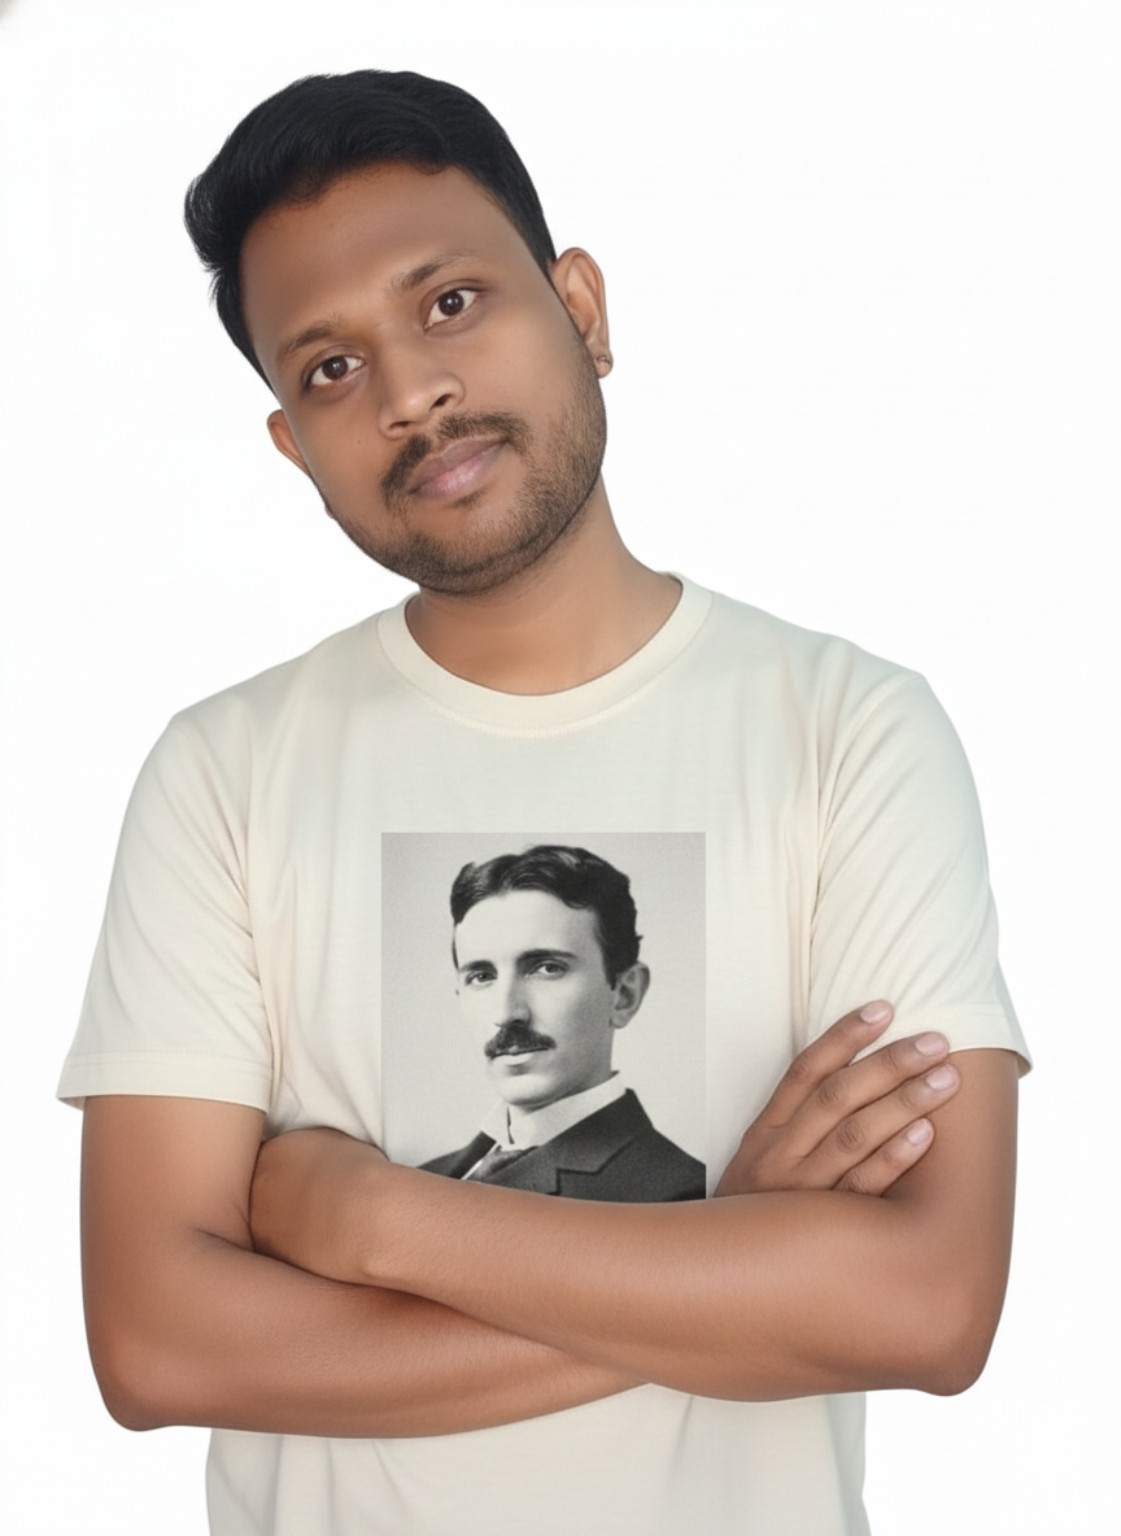
\includegraphics[width=2.3cm,height=2.3cm,keepaspectratio=false,trim=60 260 60 0,clip]{img/photo_src}};
  \draw[gilt,line width=1.2pt] (ph.south west) rectangle (ph.north east);
  \node[anchor=west,align=left] at ($(ph.east)+(0.35cm,0)$) {%
    {\color{navy}\fontsize{15}{18}\selectfont\scshape Sumeet Birajadar}\\[2pt]
    {\color{crimson}\small\itshape Founder \& Physics Mentor}\\
    {\color{ink}\small\scshape Science Monk}};
  \node[anchor=south east,align=right] at ($(current page.south east)+(-4.4cm,2.7cm)$) {%
    {\color{ink}\footnotesize\itshape\textquotedblleft Appa Deepo Bhava\textquotedblright}\\
    {\color{gilt}\footnotesize\scshape Learn \textperiodcentered{} Think \textperiodcentered{} Excel}};
\end{tikzpicture}
\null
\clearpage
\global\watermarktrue
